\documentclass[letterpaper, 10 pt, conference]{ieeeconf}
\IEEEoverridecommandlockouts
\overrideIEEEmargins
\usepackage[T1]{fontenc}
\usepackage{times,amsmath,amssymb,graphicx,booktabs,cite,url}
\usepackage[hidelinks,pdfauthor={},pdftitle={Reconstructing Cartesian Controller Targets from Replay Telemetry}]{hyperref}
\ifdefined\pdfminorversion\pdfminorversion=5\fi
\title{\LARGE\bf Reconstructing Cartesian Controller Targets\\ from Replay Telemetry}
\author{\phantom{Anonymous Author}}
\begin{document}
\maketitle
\thispagestyle{empty}
\pagestyle{empty}
\begin{abstract}
A replay program needs the target around which the controller will interpret its next displacement. A log of sent commands may leave that target ambiguous if the receiver suppresses, attenuates or delays an input. We give conditions under which a target sample or an application acknowledgment identifies the current command origin. When several origins remain possible, we test whether a proposed rewrite reduces squared target error for every origin in a bounding box. Across 36 simulated Sawyer layouts, the test admitted 658 of 12,474 candidate rewrites. All 560 that reached the controller reduced error on that write, although the guarded and unguarded policies completed the same 144 trials. In a software test of a Franka equilibrium filter, the acknowledged application cycles of 120 commands sufficed to reconstruct 5,400 updates to numerical precision. In two cohorts of physical DROID recordings, the stored command-status flag differed between observation and action sampling on 81 of 2,610 and 176 of 4,551 retained rows. These results specify what a replay interface must record before it can use a status flag to reconstruct a target or certify a change to the next command.
\end{abstract}
\begin{keywords}Motion Control, Performance Evaluation and Benchmarking.\end{keywords}

\section{Introduction}
A replay program sends a Cartesian displacement at one control cycle. The receiver may apply it later, replace it with zero, or scale its magnitude. All three events leave the same entry in the sender's log. If the next displacement starts at the target stored by the receiver, the replay program needs to distinguish these histories before it can compute the next target. Knowing which cycle applied a command can resolve the ambiguity when the receiver's update law is known (Fig.~\ref{fig:origin}).
\begin{figure}[t]
\centering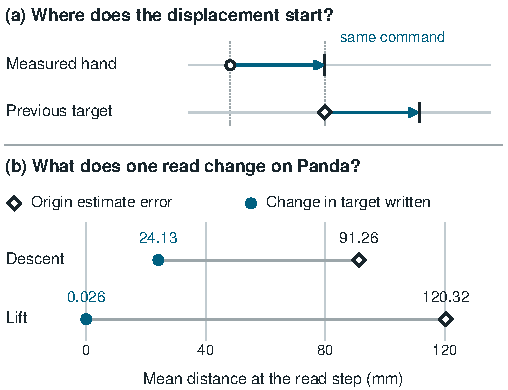
\includegraphics[width=\columnwidth]{figures/origin-readback.pdf}
\caption{(a) A replay decision uses the information available before a write. A known origin can be used directly. If several origins remain, the program tests a candidate against all of them and checks the resulting write when delivered. (b) Each marker shows one software run of the Franka equilibrium filter. Inferring the application cycle from send time produced larger reconstruction errors when callbacks were serviced every ten cycles. Application-cycle acknowledgments gave errors below $10^{-6}$\,mm in both settings.}\label{fig:origin}
\end{figure}
Action definitions vary across robot datasets and can affect transfer~\cite{openx2024,aljalbout2024action}. ManiSkill2 distinguishes measured and desired command references when converting demonstrations~\cite{gu2023maniskill2}. MimicGen converts target poses into bounded actions~\cite{mimicgen2023}. These conversions depend on the reference used by the receiver. Even when the source convention is known, the destination may have applied a different sequence of inputs.

Reference governors and reactive trajectory adaptation address command constraints and feedback during execution~\cite{governor,vochten2021}. Event-triggered control and estimation relate communication to a control or estimation objective~\cite{tabuada,trimpe}. Input acknowledgments can inform a controller about losses~\cite{schenato}, and event-triggered communication has supported cooperative manipulation~\cite{cooperative}. These approaches motivate asking what the receiver actually acknowledges. A forwarded message can have a known cycle but an unknown magnitude. A target message can have a known value but arrive several control steps after sampling.

We trace the information needed for reconstruction from a physical log field to a controller update, then to a proposed change in the next command. We check field timing in DROID recordings and reconstruct a Franka software filter from data available at each decision. For ambiguous origins we derive a sufficient condition for a specific rewrite and check its delivered writes in closed-loop simulation. Paired replay trials establish how these write-level findings relate to hand motion and task completion. All manipulation outcomes are measured in simulation.
\section{Reconstructing and Testing a Target Write}
\subsection{The command seen by the receiving controller}
Let $x_t^\star$ and $x_t$ denote the demonstrated and replayed hand positions just before command $t$. The source command specifies a translation $a_t$ in metres after action scaling, and writes the target $g_t^\star$. The recorded hand need not have reached that target. We score the hand against the recorded hand at the same post-step time and score the target separately at the instant it is written.

Let $b_t$ be the command origin, $s$ the per-axis limits, and $C$ the workspace clip. A legal displacement $d$ writes
\begin{equation}
 F(b_t,d)=C(b_t+d),\quad -s\le d\le s .\label{eq:setter}
\end{equation}
Fetch uses the measured gripper position as $b_t$. Sawyer uses its last written target. On the source tape, Fetch's hand and command determine $g_t^\star$. On Sawyer the initial target and the commands applied during the clean demonstration determine it recursively. A replay read supplies the current \emph{destination} origin. It leaves the source tape unchanged.

To retain the lag between hand and target in the demonstration, we request $h_t=g_t^\star+k(x_t^\star-x_t)$, where $k$ is the hand feedback gain. For an origin estimate $b$, project $h_t$ onto the reachable box $[C(b-s),C(b+s)]$ to obtain $q$. Sending $d=\operatorname{clip}_{[-s,s]}(q-b)$ realizes $q$ if $b$ is the true origin and the command reaches the setter.

For an accumulating receiver, let $u_j$ be the increment actually applied at cycle $j$. Its origin satisfies $b_{j+1}=C(b_j+u_j)$. Knowing an origin at cycle $\tau$ and the applied increments through $t-1$ identifies $b_t$ by iteration. A received bit supplies $u_j$ when it identifies the application cycle and selects between two known increments, such as the submitted command and zero. A forwarded input of unknown amplitude leaves multiple possibilities. A delayed target packet provides $b_\tau$ at its sample cycle. To use it at $t$, propagate all updates between those cycles. Clipping can make distinct input histories meet at the same origin, so unique knowledge of every past input is sufficient but can be unnecessary.

\subsection{A tight error floor for two compatible histories}
Suppose the observations and sent commands leave two possible origins, $b$ and $b-v$. For example, a hidden overwrite could replace $v$ by zero. Take $h=b$ and assume the workspace is locally inactive and $v$ is an admissible displacement. Sending a common $d$ incurs Euclidean errors $\|d\|_2$ and $\|d-v\|_2$. By the triangle inequality their larger value is at least $\|v\|_2/2$, attained by $d=v/2$. A program that insists on zero error for the first history must send $d=0$ and incur $\|v\|_2$ on the other. An exact read allows a different command in each history and zero error on both. The ambiguity lasts only as long as both histories remain compatible with the available observations.

We tested this construction on Sawyer's native setter at 16 reset states across push and drawer-open. We held the hand, joint positions and joint velocities fixed, separated the stored origins along one axis by 2, 5 or 8\,mm, and issued zero, midpoint and exact corrections. Across 144 matched problems (864 writes), the largest absolute difference from the predicted residual was below $10^{-10}$\,mm (Fig.~\ref{fig:ambiguity}).
\begin{figure}[t]
\centering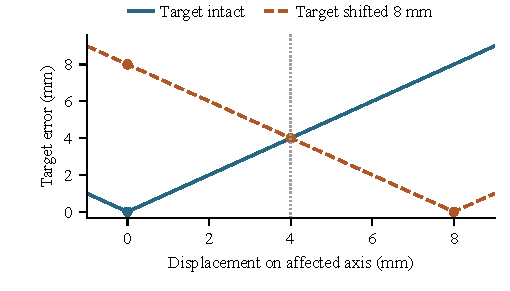
\includegraphics[width=\columnwidth]{figures/ambiguity.pdf}
\caption{One native Sawyer setter state with two origins 8\,mm apart. Lines show the predicted write errors for a shared displacement on one axis. The dots show native setter writes. A 4\,mm midpoint gives the smallest worst error without a read. Reading the origin lets the program choose the zero-error action for each history.}\label{fig:ambiguity}
\end{figure}

\subsection{The value of a read under action and workspace limits}
Let $B=[L,H]$ contain the origins compatible with the available history, let $A=[-s,s]$, and let $\ell(b,d)=\|F(b,d)-h\|_2^2$. If an exact read arrives before the next command and that command reaches the setter, the smallest worst-case squared errors are
\begin{equation}
 V_0=\min_{d\in A}\max_{b\in B}\ell(b,d),\quad
 V_1=\max_{b\in B}\min_{d\in A}\ell(b,d).\label{eq:value}
\end{equation}
Without a read one command must serve every origin. With a read the replay can choose a command for the observed origin. Thus $V_0-V_1\geq0$ quantifies the reduction in worst error on this write. The two values are exact on $B$. If $B$ is an outer box for a correlated set of histories, their difference need not equal the value on that history set. Its horizon is one delivered write.

The box constraints and squared loss separate across axes. On one axis the worst absolute residual for a fixed $d$ is $\max\{h-C(L+d),C(H+d)-h\}$. The first term decreases weakly with $d$ and the second increases weakly. Their crossing minimizes the maximum, with the corresponding action endpoint optimal when they do not cross on $A$. For a known $b$ the least absolute residual is the distance from $h$ to $[C(b-s),C(b+s)]$. Its maximum over $B$ occurs at $L$ or $H$. Let $r_1$ denote that maximum endpoint distance. The no-read policy matches the informed policy's worst error on this axis precisely when a legal $d$ satisfies
\begin{equation}
 C(L+d)\ge h-r_1,\qquad C(H+d)\le h+r_1 .\label{eq:criterion}
\end{equation}
These inequalities place the entire interval of possible writes inside the informed policy's worst-error tolerance. If they are infeasible, a read strictly improves the one-axis worst error. Squaring and summing the per-axis distances gives the two values in~\eqref{eq:value}. We checked the calculation on 1,088 native Sawyer writes, including workspace and action limits. With an 18\,mm origin half-width and a 10\,mm action limit, a read reduced the worst distance from 18 to 8\,mm.

\subsection{A sufficient condition for changing a command}
A replay program can also ask whether a proposed rewrite $d_1$ improves on the recorded displacement $d_0$ for \emph{every} compatible origin. When a submitted displacement may be executed or replaced by zero, propagate $B$ through both clipped updates and take their coordinatewise hull. A read collapses $B$ to the measured target. The hull contains every compatible origin under the stated fault model, and may include impossible histories. Define
\begin{equation}
 D=\max_{b\in B}\big[\ell(b,d_1)-\ell(b,d_0)\big].\label{eq:guard}
\end{equation}
If $D<-\delta$, any delivered $d_1$ reduces squared target error by more than $\delta$ throughout $B$. To compute $D$ on each axis, evaluate the origin interval endpoints, the four workspace breakpoints for $b+d_0,b+d_1$, and $h-d_0,h-d_1$ when inside the interval. Between breakpoints, each target is constant or affine with slope one. The loss difference is constant or affine when both slopes agree. With one active slope its only possible interior extremum is where the active target equals $h$. Summing coordinate maxima is therefore exact on the box and takes linear time in the number of axes. We use $\delta=10^{-12}\,\mathrm{m}^2$. For a known interval of desired targets on each axis, both endpoints suffice because the difference is affine in $h$ for fixed $b$.

We tested the candidate-specific guarantee on 36 previously unused Sawyer layouts, 12 per task. Each underwent the four replay conditions described in Sec.~\ref{sec:protocol}. We compared copying the recorded displacement against the event policy's proposed rewrite at the same origin and desired target. The guard admitted 658 of 12,474 proposals. Of these, 98 were suppressed. All 560 that reached the setter strictly reduced squared write error at the realized origin. Guarded and unguarded policies both succeeded on all 144 trials, but the guard requested 125 reads versus 115 and produced greater mean hand-path RMS error (2.96 versus 2.64\,mm). Thus verified improvements on individual writes coexisted with worse tracking over the episode.

\section{Which Telemetry Identifies the Target?}
\subsection{Inspecting the field at its producer}
We examined two sets of physical demonstration logs to ask whether a replay program could identify the target accepted by the receiver. In 12 DROID recordings~\cite{droid2024}, the observation-time and action-time values of \texttt{prev\_command\_successful} differed on 81 of 2,610 non-skipped rows. A second set of 13 recordings from disjoint site--date pairs had 176 differences in 4,551 rows, including 105 in one recording. All 25 recordings stored calculated Cartesian commands. None included the Franka native commanded-pose field or rolling reception rate. In the archived Polymetis client, a change in desired torque sets the status flag.\footnote{\href{https://github.com/facebookresearch/fairo/blob/0a01a7fa7a7c65b2f9a3aebf5e79040940daf9d2/polymetis/polymetis/src/clients/franka_panda_client/franka_panda_client.cpp}{Polymetis Franka client, archived implementation.}} Reconstructing a target therefore requires the producer, timestamp and meaning of each field.

\subsection{Reading the application cycle of a software filter}
To isolate the information provided by application time, we compiled the translational equilibrium filter from the Franka impedance example into a local cross-process harness.\footnote{\href{https://github.com/frankarobotics/franka_ros/blob/35e1f654426e04bc9f83b73af4ab68a3fb145c84/franka_example_controllers/src/cartesian_impedance_example_controller.cpp}{Franka Cartesian impedance example, pinned implementation.}} The client and controller communicated over local UDP. The controller processed callbacks every cycle or every ten cycles, with three repetitions per setting and 900 updates per run. Each observer used only messages received by the decision time. Across 5,400 updates, the application-cycle acknowledgments for all 120 commands arrived before the first affected target sample, allowing reconstruction to numerical precision. Across the three repetitions, using send time to infer application time gave target RMS errors of 0.074--0.144\,mm with callbacks every cycle and 0.585--0.791\,mm with callbacks every ten cycles (Fig.~\ref{fig:origin}b). Median round-trip times for requested targets ranged from 0.802 to 1.487\,ms across six runs. Adding the private equilibrium to 27 status messages per run cost 1,675--1,712 payload bytes with zero extra requests. Both the field and the acknowledgments were supplied by our harness.

\subsection{When does a bit identify the applied input?}
An execution acknowledgment can substitute for a target value if it identifies the applied displacement. On 24 fresh Sawyer layouts we sent either three execution bits or the stored target every three steps, with both packets arriving two steps later. For binary forwarding or substitution by zero, knowledge of the initial target, applied increments and workspace clip was sufficient. Both streams produced identical trajectories in all 96 paired conditions. When five accepted translations were subsequently attenuated to one quarter, the bits continued to report forwarding. Mean hand RMS then reached 10.126\,mm with execution bits, 5.149\,mm with targets and 6.679\,mm with empty packets. Each policy still completed all 48 attenuation trials. In 5,025 of 7,200 decisions under attenuation, interpreting a forwarded command as full execution caused the predicted origin box to exclude the true origin. These are correlated control steps from 24 layouts.

\section{Paired Replay Protocol}
\subsection{Demonstrations, interventions and outcomes}
For each layout, we record a scripted demonstration, restore the initial state and replay to a fixed horizon. Policies receive the source tape and measured hand positions. Gripper commands pass through unchanged. We use object state, fault labels and task predicates to construct and score the experiments. We verify initial states and source tapes across paired policies and retain failed demonstrations.

Fetch push and pick-and-place use Gymnasium-Robotics 1.4.2 and MuJoCo 3.3.7, with a 50-step horizon and 50\,mm per-axis translation scale~\cite{plappert2018fetch}. Meta-World 3.1.1 and MuJoCo 3.3.0 use 10\,mm increments relative to Sawyer's previous mocap target~\cite{yu2020metaworld,mclean2025metaworld}. We use its released push, pick-place and drawer-open experts and evaluate at step 150. Each layout undergoes four conditions: clean replay, five consecutive translations overwritten by zero, a 20\,N hand force along negative world $y$ for three steps, and both interventions. We draw onset times from steps 7--29 on Fetch and 8--65 on Sawyer. All policies in a pair share those times. Fault type and onset are hidden during ordinary replay.

The initial comparison uses 24 held-out layouts per task, or 120 layouts and 3,360 branch executions. Seven clean Fetch push demonstrations miss the task goal and remain in the sample. Follow-up comparisons use separately identified cohorts. We score the native success predicate at the \emph{last} step. For each episode the hand-path RMS error is $\sqrt{T^{-1}\sum_{t=1}^{T}\|x_t-x_t^\star\|_2^2}$. We average this error across episodes. Paired bootstrap intervals resample layouts within each task, carrying all conditions for each layout together. Equal task and intervention weights define this stress test. They have no assumed deployment frequency.

\subsection{Information supplied to each policy}
A command-history policy starts with the known origin and updates it using the commands it sends. An undetected overwrite breaks that recursion. A target read resets the estimate. In the original event policy, two consecutive hand deviations above 5\,mm trigger a read, with a ten-step cooldown and at most two reads per trial. A scheduled policy reads at steps 16 and 32 on Fetch or 50 and 100 on Sawyer. The Sawyer times and $k=0.5$ came from a development comparison of three schedules and two gains. A lower-cost variant checks the residual at the two scheduled times only.

The hand-based observer uses the recorded offset between source hand and source origin. Let $\tilde b_t$ be the live origin predicted from previous estimates and sent commands, and let $b_t^\star$ be the source origin. The correction is
\begin{equation}
 \hat b_t=C\!\left(\tilde b_t+0.25\big[x_t+(b_t^\star-x_t^\star)-\tilde b_t\big]\right).\label{eq:observer}
\end{equation}
It places the recorded offset at the current hand, blends this candidate with the prediction, and propagates the updated estimate using its next submitted command. The read and zero-read branches share this observer, including its gain. We froze it after an eight-layout development trial. It assumes access to a clean source tape, an initialized target and time-aligned hand measurements.

For the limited-resolution comparisons we delay both hand measurements and requested targets by two steps. We propagate a delayed target with submitted commands and transport the last measured hand residual along the demonstration. Only the replay's live hand is rounded to a 1 or 5\,mm grid in world coordinates. The event policy may read once after two steps above 5\,mm. Before testing new layouts at 5\,mm, we fix a read at step 41 (the median development event time) and define a second schedule by permuting the 96 development event times independently of the new motions.

\section{Reconstruction in Simulated Replay}
The Fetch, Sawyer observer, coarse-measurement and Panda cohorts also appear in a companion study of contact outcomes. Here they test the consequences of recovering the command origin. They represent shared episodes across the two analyses.
\subsection{Re-encoding at a measured origin}
After the five-step override, direct copying succeeded on 22 of 48 Fetch layouts. Re-encoding the desired target from the measured hand at $k=0$ succeeded on 41 of 48, matching the number of successful source demonstrations. It rescued ten push and nine pick-and-place trials without losing any or requesting the controller target. Figure~\ref{fig:fetch} shows one rescued push. Under force alone re-encoding lost one push that direct copying completed, even though across force trials the mean hand-path RMS error fell from 0.033 to 0.005\,mm. Improving hand tracking does not ensure the cube finishes closer to its goal.
\begin{figure}[t]
\centering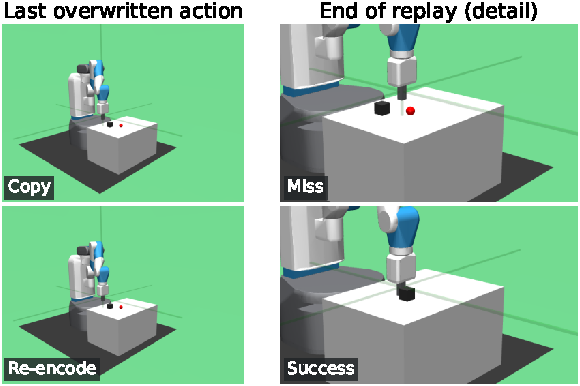
\includegraphics[width=\columnwidth]{figures/fetch-example.pdf}
\caption{Replay of the same FetchPush layout after five overwritten translations. At tick 14 the final overwrite occurs (left). At the last tick the cube is 134.4\,mm from the goal under direct copying and 23.3\,mm from it after re-encoding (right, enlarged). We show the lowest-index held-out push layout rescued by re-encoding.}\label{fig:fetch}
\end{figure}

\subsection{How much does Sawyer's hand already reveal?}
The clearest comparison holds the observer fixed and varies access to the internal target. On 36 fresh Sawyer layouts (12 per task), the hand-based observer recovered six trials lost by command history alone, with no losses. Reading on events while retaining command history recovered exactly the same six. Adding event reads to the hand-based observer changed none of the 144 paired terminal outcomes (Table~\ref{tab:observer}). The 123 extra reads reduced mean hand-path RMS error by 0.039\,mm (paired 95\% layout-bootstrap interval for the reduction, 0.012--0.068\,mm). Four push trials still failed with either observer branch.
\begin{table}[t]\centering
\caption{Sawyer policies on the same 36 layouts and four conditions per layout. Reads are total extra requests. RMS is the mean of per-episode hand-path errors.}\label{tab:observer}
\begin{tabular}{@{}lrrr@{}}\toprule
Origin estimate and read policy & Success & Reads & RMS (mm)\\\midrule
Command history only & 134/144 & 0 & 6.497\\
Command history + event & 140/144 & 112 & 2.734\\
Hand-based observer & 140/144 & 0 & 2.830\\
Observer + event & 140/144 & 123 & 2.790\\
Observer + gated fixed times & 140/144 & 32 & 2.829\\\bottomrule
\end{tabular}
\end{table}

Earlier schedule comparisons illustrate why the choice of baseline matters. With command history and hand feedback gain $k=0.5$, event and scheduled reads yielded 192/192 and 190/192 successes on push and pick-place, using 160 and 384 reads, respectively. The two event-only successes arose on a single pick-place layout, under the overwrite and combined conditions (Fig.~\ref{fig:sawyer}). The difference was 1.04 percentage points (95\% layout-bootstrap interval, 0.00--3.13). It fell short of the prespecified five-point gain with a positive lower confidence limit. The 96 drawer conditions agreed. At $k=0$, event reads succeeded on 192/192 compared with 166/192 for the scheduled reads. The larger difference applies to this weaker hand-feedback comparator.
\begin{figure}[t]
\centering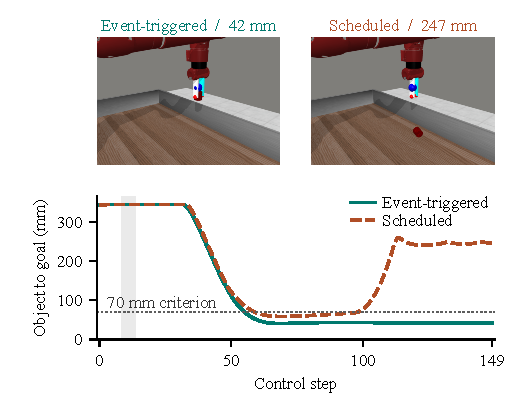
\includegraphics[width=\columnwidth]{figures/sawyer-case.pdf}
\caption{The single Sawyer pick-place layout accounting for both event-only successes against scheduled reads at $k=0.5$. During the overwrite trial both policies brought the object within 70\,mm of its goal. At the final step the event branch was 42.3\,mm away and the scheduled branch 246.7\,mm away.}\label{fig:sawyer}
\end{figure}

Two tests distinguish knowledge of fault timing from information available online. On 24 further layouts, an immediate read after an override timed to source contact and a no-read observer each completed 48/48 trials. In a separate 24-layout cohort, an online trigger requested a read when two available candidate commands differed by more than 2.5\,mm for two steps. At two-step delay both branches completed 94/96. The 48 extra requests raised mean hand-path RMS error from 4.429 to 4.504\,mm.

\subsection{Changing the command origin on the same Panda}
To compare origins on one robot, we switched the native Cartesian controller of one simulated Panda between measured and accumulating origins in robosuite 1.5.2 (MuJoCo 3.3.7)~\cite{robosuite2020}. We used the same eight initial physical layouts in both modes and generated a separate clean source for each mode and layout. Within a mode the policies replayed the same source. Cross-mode differences therefore include any change in the source trajectory. At 20\,Hz the source closed the gripper at step 60 and raised it at step 80. We overwrote five translations during descent (steps 35--39) or lift (80--84). One observer branch read once immediately after the scheduled override. This timing tests the effect of knowing the origin at that instant. Success required the cube center to finish more than 40\,mm above the table at step 120. All 16 sources succeeded. We retained all 192 replays, including failures.

After the descent override, direct copying failed on every layout in both modes. On the measured-origin controller, re-encoding from the current hand rescued all eight. On the accumulating controller, integration of submitted commands rescued none, whereas the hand-based observer and the observer with one read each rescued all eight. During lift every policy succeeded on all eight layouts. All terminal successes also held over the last 20 steps.
\begin{figure}[t]
\centering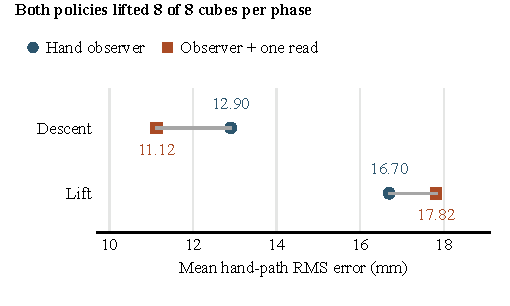
\includegraphics[width=\columnwidth]{figures/replay-comparison.pdf}
\caption{Paired replays on the accumulating Panda controller. A read after the descent override reduced mean hand-path RMS error from 12.90 to 11.12\,mm. During lift it increased the error from 16.70 to 17.82\,mm. Both observer policies lifted the cube on all eight layouts in each phase.}\label{fig:panda}
\end{figure}

During lift both observer branches requested maximum upward translation in all eight layouts. Reading the target then changed mean hand-path RMS from 16.70 to 17.82\,mm, while the eight terminal outcomes agreed (Fig.~\ref{fig:panda}).

\subsection{Three rescues with coarse hand feedback}
With two-step observation latency, unrounded and 1\,mm hand observations yielded 94/96 Sawyer successes with and without an event read on 24 push and pick-place layouts. On a 5\,mm grid the event policy achieved 94/96 versus 91/96 for the observer alone. All three extra successes came from two push layouts. The policy requested on all 96 development episodes, including all 24 clean episodes.

On 24 new layouts with the 5\,mm grid, the zero-read, event, fixed-time and permuted-time policies each succeeded on 96/96. They used 0, 94, 96 and 96 reads and had mean hand RMS errors of 6.409, 6.227, 6.293 and 6.399\,mm, respectively. The development rescues did not recur (Fig.~\ref{fig:confirm}). The ceiling in the new cohort limits inference about rarer conditions in which a read might rescue contact.

\begin{figure}[t]
\centering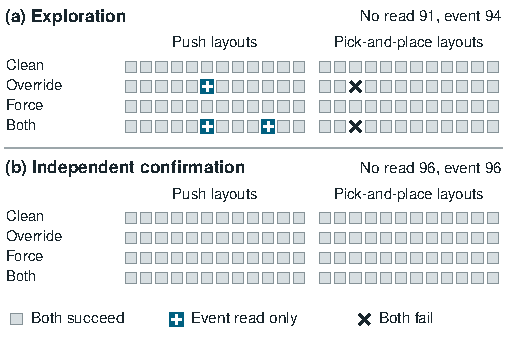
\includegraphics[width=\columnwidth]{figures/sawyer-confirmation.pdf}
\caption{Paired terminal outcomes with 5\,mm Sawyer hand observations. Each column is one layout and each row one intervention. Three event-only successes came from two development layouts. The four frozen policies each succeeded on every confirmation trial.}\label{fig:confirm}
\end{figure}

\section{Discussion}
The first question for a replay implementation is which state its displacement updates. A measured-origin controller exposes that state through the hand observation. For an accumulating controller the initial target, update law and timed sequence of applied increments suffice. A sampled target anchors that reconstruction at its sample cycle. If later inputs are ambiguous, the uncertainty grows again before the packet arrives. An execution bit settles the ambiguity only to the extent that its producer identifies the applied input under the model in use. The local Franka experiment illustrates the value of an application-cycle field when its update law and parameters are known. DROID illustrates the difficulty of identifying an equivalent field in an archived physical demonstration.

A program can still decide to change a command with an uncertain origin. The guarantee in~\eqref{eq:guard} compares two displacements at the same origin and desired target for one delivered write. Even a certified improvement on that write may increase trajectory error, consume more reads or leave object placement unchanged. Synchronized physical replay with independently logged applied inputs and object outcomes would test how much these distinctions matter under real sensing and communication delays~\cite{li2025simpler}.

The experiments use scripted time-aligned sources and Cartesian translations. The origin set depends on the assumed fault model. A forwarding flag interpreted as proof of full application can exclude the true origin when inputs are attenuated. The quantized-hand experiments model deterministic coordinate rounding. The all-success confirmation cohort limits inference about uncommon rescues. Costs of reading also depend on whether the receiver already streams the target. These conditions delimit when a replay implementation can use the guarantees reported here.

\section*{Acknowledgment}
OpenAI Codex assisted with experimental design, implementation and execution, literature checks, analysis, figure code and drafting throughout the article. The robot images in Figs.~\ref{fig:fetch} and~\ref{fig:sawyer} are native simulation renders.

\bibliographystyle{IEEEtran}
\bibliography{references}
\end{document}
